\chapter{Finite-size scaling of the exponents across topologies}
\label{app:scaling}

Section~\ref{sec:growing-finite-size} reported that the multiscaling ratios are converged in
system size while the size--variance exponent $\beta$ drifts, and gave the drift for the
power-law-$2.5$ graph. Because the drift is the sharpest quantitative caveat on the model, this
appendix documents it for every topology of Section~\ref{sec:growing-graph}, so that what is a
finite-size transient and what is a converged prediction can be told apart at a glance.
Figure~\ref{fig:scaling-topology} and Table~\ref{tab:scaling} give the size--variance exponent
and the highest multiscaling ratio $\zeta_4/\zeta_1$ against $N$, at the fixed dilution
$C = N/40$, for each degree distribution. The fully-connected graph is dense and cannot be
carried past $N = 16000$ on the available hardware; the regular graph, homogeneous but sparse,
provides the homogeneous control at the largest sizes.

Two patterns separate cleanly. The multiscaling ratio (right panel) is flat in $N$ for every
topology to within its error: the homogeneous graphs sit on the fixed-shape value $4$ at every
size, and each heterogeneous graph holds its own value ($\zeta_4/\zeta_1 \approx 3.4$ for the
power-law-$3.5$ graph, $\approx 3.1$ for power-law-$2.5$, $\approx 2.7$ for power-law-$2.2$)
across the whole range from $N = 8000$ to $32000$. The multiscaling is thus a genuine
thermodynamic property of each ensemble, set by the degree distribution and not by the system
size, and the empirical value $2.9$ is bracketed between the power-law-$2.5$ and
power-law-$2.2$ graphs at every $N$ measured.

The size--variance exponent (left panel) behaves differently. It drifts upward with $N$ for
every topology, but the drift and its limit are organized by the degree distribution. On the
homogeneous graphs $\beta$ is already at or close to $1$ and barely moves: the fully-connected graph holds
$1.02$, the regular graph creeps from $0.94$ to $0.99$. As the degree distribution broadens the
exponent both drops and, for the most heterogeneous graph, settles: the power-law-$2.2$ graph
rises from $0.16$ at $N = 8000$ to $0.22$ at $16000$ and $0.23$ at $32000$, the last two
agreeing within their errors, so that its exponent has essentially converged just above the
empirical band $0.15$--$0.20$. The power-law-$2.5$ and power-law-$3.5$ graphs are still drifting
at $N = 32000$ and their limits are not pinned by these sizes. What the sweep establishes is
therefore not a single matched exponent but a monotonic control: the degree-tail exponent sets
where $\beta$ lands, spanning the whole range from $1$ down through the empirical band, while it
leaves the multiscaling ratio fixed. The size-conditioned \emph{shape} is the converged
prediction of the model; the absolute exponent is a finite-size quantity whose large-$N$ value
the topology tunes toward, and in the most heterogeneous case into the neighbourhood of, the
data.

\begin{figure}[htbp]
    \centering
    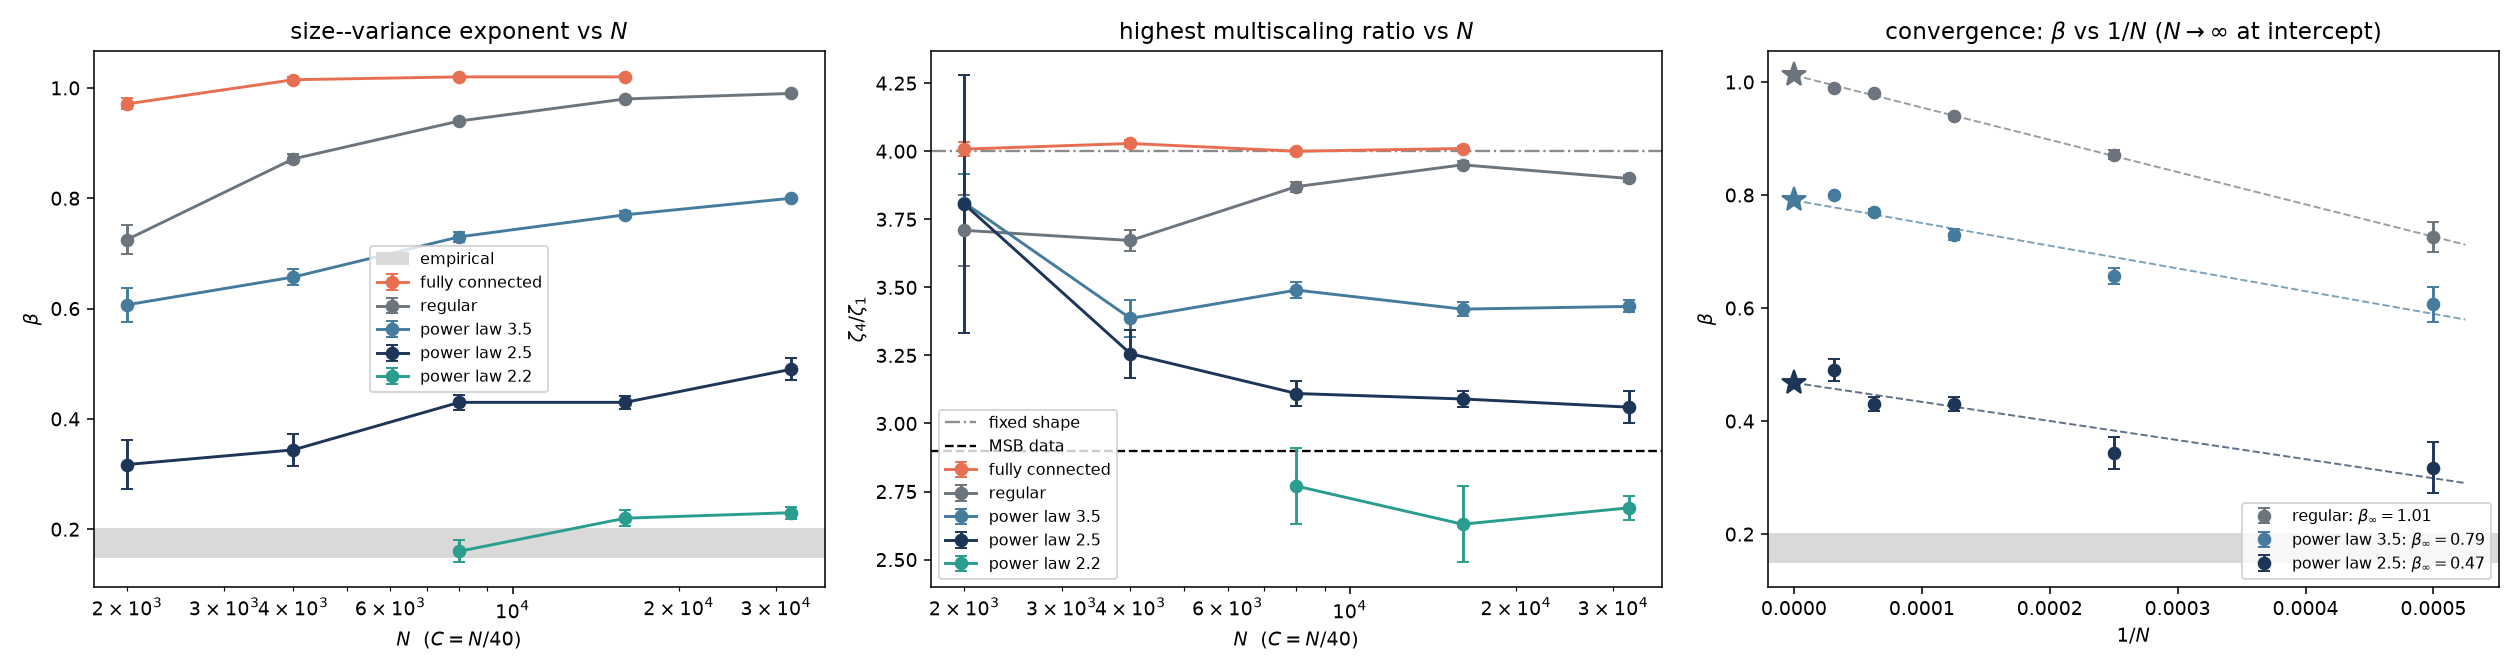
\includegraphics[width=\linewidth]{meandeg_scaling_topology.png}
    \caption{Finite-size scaling of the exponents at fixed dilution $C = N/40$, for the five
    degree distributions of Section~\ref{sec:growing-graph} (12--20 economies per point).
    \panel{Left}: the size--variance exponent $\beta$ against $N$; it drifts upward for every
    topology, but the drift shrinks and the value falls as the degree distribution broadens,
    from $\beta \approx 1$ on the homogeneous graphs to $\beta \approx 0.23$, converged, on the
    power-law-$2.2$ graph, just above the empirical band. \panel{Right}: the highest
    multiscaling ratio $\zeta_4/\zeta_1$ against $N$; flat in $N$ for every topology, set by the
    degree distribution, with the empirical value bracketed between the power-law-$2.5$ and
    power-law-$2.2$ graphs. The fully-connected graph, dense, is not run beyond $N = 16000$.}
    \label{fig:scaling-topology}
\end{figure}

\begin{table}[htbp]
    \centering
    \begin{tabular}{llccc}
        \hline
        & & $N=8000$ & $N=16000$ & $N=32000$ \\
        \hline
        \multirow{5}{*}{$\beta$}
          & fully connected & $1.02$ & $1.02$ & n/a \\
          & regular         & $0.94$ & $0.98$ & $0.99$ \\
          & power law $3.5$ & $0.73$ & $0.77$ & $0.80$ \\
          & power law $2.5$ & $0.43$ & $0.43$ & $0.49$ \\
          & power law $2.2$ & $0.16$ & $0.22$ & $0.23$ \\
        \hline
        \multirow{5}{*}{$\zeta_4/\zeta_1$}
          & fully connected & $4.00$ & $4.01$ & n/a \\
          & regular         & $3.87$ & $3.95$ & $3.90$ \\
          & power law $3.5$ & $3.49$ & $3.42$ & $3.43$ \\
          & power law $2.5$ & $3.11$ & $3.09$ & $3.06$ \\
          & power law $2.2$ & $2.77$ & $2.63$ & $2.69$ \\
        \hline
    \end{tabular}
    \caption{The size--variance exponent $\beta$ and the highest multiscaling ratio
    $\zeta_4/\zeta_1$ against system size, at $C = N/40$, for each degree distribution
    (standard errors $\le 0.02$ on $\beta$ and $\le 0.14$ on the ratio; the empirical values are
    $\beta \approx 0.15$--$0.20$ and $\zeta_4/\zeta_1 \approx 2.9$). The ratio is flat in $N$ for
    every topology; $\beta$ drifts upward but its value is set by the degree distribution, and
    for the power-law-$2.2$ graph it has converged just above the empirical band. The
    ensembles here are independent of those behind the main-text figures; where the same
    quantity appears in both, the values agree within the quoted errors. The
    fully-connected graph is dense and is not run at $N = 32000$.}
    \label{tab:scaling}
\end{table}
